\section{Remote Control and Communication}

The remote control and communication system of the two-wheeled self-balancing robot was designed to enable seamless and reliable interaction between the user and the robot. For this purpose, we integrated the BT16 Bluetooth UART Module, which provided a robust wireless communication link.

\subsection{Bluetooth Module Integration}
The BT16 Bluetooth UART Module is a high-performance component based on the Airoha ABI 602 chipset, compliant with the Bluetooth 4.2 BLE standard. It interfaces with the microcontroller via UART, ensuring efficient bidirectional data transmission. The module supports GATT-based communication through an integrated transparent data transmission service, enabling seamless and reliable Bluetooth connectivity.

A key feature of the BT16 module is its \textit{serial command mode}, which allows direct configuration and control via UART commands. Users can modify essential parameters, such as the UUID, device name, and connection settings, facilitating flexible integration into various applications.


\begin{figure}[H]
	\centering
	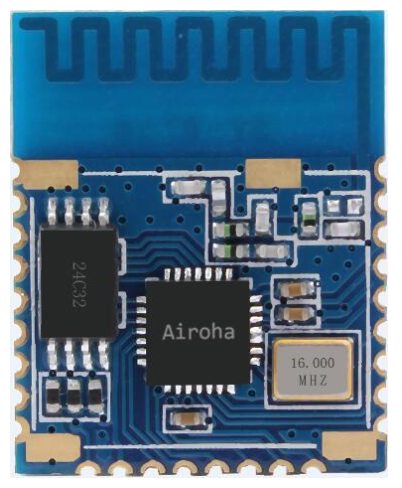
\includegraphics[height=3cm]{assets/BT16Module.png}
	\caption{Ultrasonic distance sensor by  Sparkfun electronics \cite{bluetooth_module}.}
	\label{fig:bluetooth}
\end{figure}



\subsection{Custom Communication Protocol}
A custom communication protocol was developed to manage the exchange of control commands and telemetry data, which is structured around well-defined command and telemetry packets, implemented in \texttt{comm.hpp}. These packets support multiple data formats, ensuring compatibility with various communication protocols. The functions responsible for sending and receiving telemetry data are listed in Tables~\ref{tab:uart_methods} and~\ref{tab:i2c_methods}.


\subsection{User Interfaces}
The user interface (UI) for the robot is designed to facilitate interactive control and real-time monitoring. It integrates command parsing, telemetry data handling, and communication protocols such as Inter-Integrated Circuit (I2C) and Universal Asynchronous Receiver-Transmitter (UART). Users can send commands to the robot and receive real-time telemetry feedback, ensuring efficient control and monitoring.

\subsection{UART Communication}
The Universal Asynchronous Receiver-Transmitter (UART) protocol is used for serial communication, typically with a Bluetooth module or a computer for debugging and remote control. The communication is initialized at a baud rate of \texttt{9600}, which is commonly used for Bluetooth modules \cite{bluetooth_module}.

\begin{table}[h]
	\centering
	\caption{UART Communication Methods}
	\begin{tabular}{|l|l|l|}
		\hline
		\textbf{Packet Type} & \textbf{Function} & \textbf{Description} \\ \hline
		\multirow{4}{*}{Command Packets} & \texttt{readUartBytes()} & Reads command data as raw bytes. \\ \cline{2-3}
		& \texttt{readUartASCII()} & Reads command data as an ASCII string. \\ \cline{2-3}
		& \texttt{sendUartBytes()} & Sends command data as raw bytes. \\ \cline{2-3}
		& \texttt{sendUartASCII()} & Sends command data as an ASCII string. \\ \hline
		\multirow{4}{*}{Telemetry Packets} & \texttt{sendUartBytes()} & Sends telemetry data as raw bytes. \\ \cline{2-3}
		& \texttt{sendUartASCII()} & Sends telemetry data as an ASCII string. \\ \cline{2-3}
		& \texttt{readUartBytes()} & Reads telemetry data as raw bytes. \\ \cline{2-3}
		& \texttt{readUartASCII()} & Reads telemetry data as an ASCII string. \\ \hline
	\end{tabular}
	\label{tab:uart_methods}
\end{table}

\subsection{I2C Communication}
Inter-Integrated Circuit (I2C) communication is used for short-range, two-wire serial communication. The robot operates as an I2C slave with a predefined address (SLAVE\_ADDR = 8), allowing it to receive commands and transmit telemetry data over the I2C bus.

\begin{table}[h]
	\centering
	\caption{I2C Communication Methods}
	\begin{tabular}{|l|l|l|}
		\hline
		\textbf{Packet Type} & \textbf{Function} & \textbf{Description} \\ \hline
		\multirow{4}{*}{Command Packets} & \texttt{sendI2CBytes(addr)} & Sends command data as raw bytes to the address. \\ \cline{2-3}
		& \texttt{sendI2CASCII(addr)} & Sends command data as ASCII to the address. \\ \cline{2-3}
		& \texttt{readI2CBytes(addr)} & Reads command data as raw bytes from the address. \\ \cline{2-3}
		& \texttt{readI2CASCII(addr)} & Reads command data as ASCII from the address. \\ \hline
		\multirow{4}{*}{Telemetry Packets} & \texttt{sendI2CBytes()} & Sends telemetry data as raw bytes. \\ \cline{2-3}
		& \texttt{sendI2CASCII()} & Sends telemetry data as ASCII. \\ \cline{2-3}
		& \texttt{readI2CBytes(addr)} & Reads telemetry data as raw bytes from the address. \\ \cline{2-3}
		& \texttt{readI2CASCII(addr)} & Reads telemetry data as ASCII from the address. \\ \hline
	\end{tabular}
	\label{tab:i2c_methods}
\end{table}

\subsection{Sending Commands}
Users can send commands to control the robot’s movement, rotation, or stop function. Commands follow a predefined structured format and can be transmitted via either I2C or UART. The available commands are listed in Table~\ref{tab:commands}.

\textbf{ASCII Format}:
The commands sent in ASCII is formatted as a comma-separated string:
\begin{lstlisting}[]
	<command>,<command_value>,<command_speed>
\end{lstlisting}

\begin{table}[H]
	\centering
	\caption{List of Commands and Corresponding Values}
	\label{tab:commands}
	\begin{tabular}{|c|c|l|}
		\hline
		\textbf{Command} & \textbf{Value} & \textbf{Description} \\ \hline
		\texttt{Stop}     & 0              & Stops the robot's movement. \\ \hline
		\texttt{Move}     & 1              & Moves forward or backward (in cm) at a given speed. \\ \hline
		\texttt{Rotate}   & 2              & Rotates the robot by a angle (in degrees) at a given speed. \\ \hline
		\texttt{INVALID}  & 3              & Represents an invalid or unrecognized command. \\ \hline
	\end{tabular}
\end{table}

\textbf{Example Command:}
\begin{itemize}
	\item Stop the robot: \texttt{0}
	\item Move forward 100 cm at 50\% speed:  \texttt{1,100,50}
	\item Rotate 90° at 30 speed\%: \texttt{2,90,30}
\end{itemize}

\subsection{Receiving Telemetry Data}
The robot continuously monitors its state and environment using onboard sensors. This data is packaged into a structured format and transmitted back to the user for real-time monitoring and feedback. Telemetry data includes:
\begin{itemize}
	\item \textbf{Yaw Angle}: The robot's current orientation in degrees.
	\item \textbf{Distance Traveled}: The total distance traveled by the robot in centimeters.
	\item \textbf{Ultrasonic Distance}: The distance to the nearest obstacle, as measured by the ultrasonic sensor in centimeters.
\end{itemize}

\textbf{ASCII Format}:
The telemetry data recieved in ASCII is formatted as a comma-separated string:
\begin{lstlisting}[]
	<yaw_angle>,<distance_traveled>,<ultrasonic_distance>
\end{lstlisting}
\textbf{Example Output}:
\begin{lstlisting}[]
	45,200,30
\end{lstlisting}

This indicates a yaw angle of 45 degrees, a distance traveled of 200 cm, and an ultrasonic reading of 30 cm.
